% ICMLDE 2026 -- revised submission
% Procedia Computer Science CRC template (Elsevier ecrc.sty)
\documentclass[3p,times,procedia]{elsarticle}
\flushbottom

\usepackage{ecrc}
\usepackage[bookmarks=false]{hyperref}
    \hypersetup{colorlinks,
      linkcolor=blue,
      citecolor=blue,
      urlcolor=blue}
\usepackage{amssymb}
\usepackage{graphicx}
\usepackage{booktabs}

\volume{00}
\firstpage{1}
\journalname{Procedia Computer Science}
\runauth{Kavinesh P et al.}
\jid{procs}

\begin{document}
\begin{frontmatter}

\dochead{5th International Conference on Machine Learning and Data Engineering}

\title{Why AI-Generated Image Detectors Fail on Modern Diffusion
Generators: A Diagnostic Study of Cross-Architecture Generalization and
Failure Modes}

\author[a]{Kavinesh P}
\author[a]{Raam Prathap R V}
\author[a]{Santhosh A S}
\author[a]{Kasam Sai Venkata Siddardha}
\author[a]{Ashish M}
\author[a]{M Anbazhagan\corref{cor1}}

\address[a]{Department of Computer Science and Engineering, Amrita School of Computing, Coimbatore 641112, Amrita Vishwa Vidyapeetham, India}

\begin{abstract}
This is a diagnostic study: it trains nothing and proposes no detector,
and instead measures how five pretrained, publicly released AI-generated
image detectors behave on five generators spanning three architecture
families, with every generator verified absent from every detector's
training data. We use 6{,}000 real and 6{,}000 generated images for
BigGAN, GLIDE, FLUX.1 and SD3, 18{,}300 per class for SDXL, and paired
subsets of 2{,}000 per class for the compression experiments. Detectors
disagree about what is hard: one fails worst on FLUX.1 (7.0\%
fake-accuracy), another on SDXL (54.6\%), two others on BigGAN (0.4\% and
9.6\%), and paired McNemar tests on identical images confirm the gaps with
one non-significant exception between two same-lineage detectors. Two
detectors trained on identical data but different architectures produce an
\emph{identical} difficulty ordering across all five generators
($\rho=+1.000$, exact $p=0.017$) while differing 37.6 points in mean
accuracy. Testing the ensembling prediction this implies, pairing a
detector with a different-lineage partner lifts worst-generator accuracy
from 9.6\% to 62.9\%, where pairing it with a same-lineage partner of
different architecture lowers it to 0.3\%. Calibration error rises with
failure severity rather than falling, reaching 0.503 where fake-accuracy
is 0.4\%, so these models stay confident and become wrong outside their
training distribution. Two measurement hazards bound every absolute number
here: a resize convention rarely specified in released code moves the same
checkpoint by over 15 points, in opposite directions for two checkpoints
trained on identical data; and because these benchmarks pair PNG generated
images against JPEG reals, re-encoding only the generated side at JPEG
quality 75 takes the best clean-data FLUX.1 detector from AUC 97.1 to
39.1, below chance, while the other four lose between 1 and 13 points.
\end{abstract}

\begin{keyword}
AI-generated image detection \sep synthetic image forensics \sep cross-generator generalization \sep diffusion models \sep adversarial training \sep calibration \sep reproducibility
\end{keyword}
\cortext[cor1]{Corresponding author: M Anbazhagan}
\end{frontmatter}

\email{m\_anbazhagan@cb.amrita.edu}

\vspace*{-6pt}

\section{Introduction}
\label{sec:intro}

A detector's accuracy number is only useful if it predicts behavior on
data the detector has not seen. A detector trained on one generator's
outputs usually loses most of its accuracy on another generator's outputs,
and the field has largely explained this with a single story: newer
generators produce artifacts that older detectors were not built to catch.
That story predicts a pattern. Detectors should fail worst on the newest
generators, and should fail in broadly similar ways.

We test the prediction by running five independently trained, publicly
released detectors against five generators spanning three architecture
families, and it does not hold. The detectors disagree about which
generator is hardest: one fails worst on FLUX.1, another on SDXL, and two
others on BigGAN, the oldest generator in the set. In the sharpest case,
one detector recovers 5{,}452 FLUX.1 images that another misses while
losing only 8 in the opposite direction, on the identical image set.
Generator age is not the variable driving detector failure; the detector's
own training distribution is.

This is a diagnostic paper: it proposes no detector and trains nothing,
and every number comes from inference over released checkpoints and
datasets.

Five contributions follow. We report a controlled generalization audit of
five detectors on five generators, with training/test overlap verified
against primary documentation rather than inferred from the accuracy
pattern such a check is meant to validate, and every gap backed by a
paired McNemar test (Section~\ref{sec:significance}). We decompose the
disagreement using two detectors trained on identical data but different
architectures, whose difficulty orderings match exactly while their
accuracy levels differ by 37.6 points (Section~\ref{sec:finding-shape}),
then test the operational prediction that follows, that detectors should
be combined for training-lineage diversity rather than architectural
diversity (Section~\ref{sec:ensemble}). We give a calibration account of
the failure mode, with per-detector reliability diagrams
(Section~\ref{sec:confidence}). Finally we report two measurement hazards
bounding how any of these numbers should be read: a resize convention that
moves the same checkpoint by more than 15 points
(Section~\ref{sec:discussion}), and a compression asymmetry built into the
benchmarks, whose size we estimate by re-encoding the generated side to
match the real side (Section~\ref{sec:compression}).

On terminology: ``deepfake'' originally named the narrower problem of face
swapping and reenactment, where the manipulated region is a face inside an
otherwise real photograph. We study the broader task of deciding whether
an entire image was synthesised, over ImageNet-style object and scene
imagery, which is more precisely called AI-generated image detection.
Nothing here is a claim about face-manipulation detection.

\section{Related Work}
\label{sec:related}

\textbf{Cross-generator generalization.} Wang et al.~\cite{wang2020cnndetect}
established the standard protocol of training on one GAN family (ProGAN)
and testing against unseen GANs. Zhu et al.'s GenImage~\cite{genimage2023}
extended it to diffusion models at million-image scale and is the training
source for three of the five detectors we evaluate. Ojha et al.'s
UniversalFakeDetect~\cite{ojha2023universal} showed that a frozen CLIP
embedding with a linear probe, trained only on ProGAN, transfers to GANs
and early diffusion models better than end-to-end training; we use it as
our CLIP-embedding baseline. Tan et al.'s NPR~\cite{tan2024npr} instead
targets neighbouring-pixel artifacts left by a generator's up-sampling
operations, and is the one detector here whose training data and detection
signal are both unrelated to CLIP. Work that keeps the CLIP embedding and
changes the head, such as C2P-CLIP~\cite{tan2025c2pclip}, or that detects
diffusion images by reconstruction error, such as
DIRE~\cite{wang2023dire}, shows that the field's usual response to the
generalization gap is architectural, rather than asking why a given
detector's training distribution predicts where it fails.

\textbf{The adversarial-training comparison.} Zhou et al.~\cite{zhou2025omat}
attribute cross-generator failure to \emph{latent prior bias}: a detector
can key on artifacts of its training generator's initial-noise sampling
rather than of the generation process, a shortcut Xu et
al.~\cite{xu2025seed} showed exists to be learned by recovering the random
seed of a diffusion model's initial noise from the generated image. Their
fix, On-Manifold Adversarial Training (OMAT), fine-tunes against
adversarially optimized initial latents of the \emph{same} training-time
generator, and their GenImage++ benchmark adds held-out subsets from
FLUX.1~\cite{flux2024} and Stable Diffusion~3~\cite{esser2024sd3}, plus
the in-the-wild Chameleon collection~\cite{yan2024chameleon}. We neither
modify nor retrain their checkpoints; we evaluate them alongside unrelated
detectors on a wider generator set, and test whether their preprocessing
choice is load-bearing, which their evaluation did not need to ask.

\textbf{Two boundaries of scope.} The detectors here are not
face-manipulation deepfake detectors, which target a local edit inside a
genuine photograph and are benchmarked on corpora such as
FaceForensics++~\cite{rossler2019ff} and Celeb-DF~\cite{li2020celebdf};
our generators synthesise every pixel, so the two settings do not share an
artifact model. And where an interpretability literature attributes
failure to spectral artifacts~\cite{qian2020f3net,frank2020frequency} or
visualises which regions drive a classifier~\cite{selvaraju2017gradcam},
we take a coarser route in Section~\ref{sec:confidence}, characterising
the predicted probability distribution and its calibration error, which
assumes nothing about which regions carry the evidence.

\section{Methodology}
\label{sec:methods}

Every result comes from running a pretrained, publicly released detector
checkpoint over a pretrained, publicly released image dataset, with no
training and no image generation. This began as a hardware constraint,
since the single 8~GB consumer GPU used throughout cannot hold a
generation pipeline and a detector at once, but it makes the pipeline
reproducible without generation infrastructure.

\subsection{Detectors}

Table~\ref{tab:detectors} lists the five detectors, spanning 2023 to 2025.
Three use a frozen CLIP~\cite{radford2021clip} ViT-L/14 encoder with a
linear (or LoRA~\cite{hu2022lora}-adapted) probe; the other two are
convolutional, one keying on pixel and up-sampling artifacts and one a
plain ResNet-50. Training composition was confirmed from each detector's
own repository documentation, and for the GenImage++ checkpoints from the
source paper (Section~\ref{sec:methods-leakage}), rather than inferred
from how well each performed.

The GenImage++ ResNet-50 was trained on exactly the same data as the
GenImage++ CLIP baseline but is a conventional CNN with no CLIP backbone,
so it is the one pair here that varies architecture while holding training
data fixed. That is what lets Section~\ref{sec:finding-shape} separate
what the training distribution does from what the representation does.

\begin{table}[h]
\caption{Detectors evaluated. All five are used as released, with no
fine-tuning performed for this study.}
\label{tab:detectors}
\begin{tabular*}{\hsize}{@{\extracolsep{\fill}}p{2.0cm}p{2.5cm}p{4.2cm}cp{0.9cm}@{}}
\toprule
Detector & Signal & Training data (verified) & Year & Source \\
\colrule
UniversalFakeDetect & CLIP ViT-L/14 embedding + linear probe & ProGAN only, 20 LSUN categories & 2023 & \cite{ojha2023universal} \\
NPR & Pixel / up-sampling artifact (ResNet-50) & ProGAN only, 4 LSUN categories & 2024 & \cite{tan2024npr} \\
GenImage++ ResNet-50 & Plain CNN classifier (no CLIP) & GenImage SDv1.4 subset only & 2025 & \cite{zhou2025omat} \\
GenImage++ CLIP & CLIP ViT-L/14 embedding + linear probe & GenImage SDv1.4 subset only & 2025 & \cite{zhou2025omat} \\
GenImage++ CLIP-LoRA (OMAT) & Same backbone + LoRA, on-manifold adversarial fine-tune & Same SDv1.4 data + 6{,}000 SDv1.4-derived adversarial examples & 2025 & \cite{zhou2025omat} \\
\botrule
\end{tabular*}
\end{table}

For the ResNet-50 the released code and the source paper disagree on input
normalization, the former routing every detector through CLIP statistics
and the latter specifying ImageNet statistics. We measured both and used
ImageNet statistics, which performed better (85.3\% versus 80.7\%
fake-accuracy on a 150-image FLUX.1 probe): a small instance of the
under-specification problem Section~\ref{sec:discussion} treats at length.

\subsection{Generators and evaluation data}
\label{sec:methods-data}

The five generators span the three generator families that account for
essentially all current open-weight image synthesis, rather than sampling
recent releases. BigGAN~\cite{brock2019biggan} is a class-conditional GAN,
the family the first generation of detectors was built against.
GLIDE~\cite{nichol2021glide} and SDXL~\cite{podell2023sdxl} are U-Net
diffusion models, early and modern, so the U-Net family contributes a
within-family contrast of four years rather than a single point. FLUX.1
and SD3 replace the U-Net denoiser with a Diffusion
Transformer~\cite{peebles2023dit}, the architecture behind most 2024--2025
open releases. Grouping by family rather than release date is itself a
result of this study (Section~\ref{sec:finding1}). Two families we do not
cover are autoregressive token-based generators and face-specific
manipulation pipelines, the second deliberately.

BigGAN and GLIDE come from the original GenImage
benchmark~\cite{genimage2023}, each evaluated against its own paired real
split. FLUX.1, SD3 and SDXL come from GenImage++~\cite{zhou2025omat},
documented by its authors as test-only, which ships fake images only;
since it has no matched reals, we use GenImage's BigGAN-subset real
training split (about 162{,}000 ImageNet images, disjoint from the 6{,}000
used as BigGAN's own paired real evaluation split) as a shared real pool
for all three. This asymmetry is forced by the dataset and we flag it
rather than leave it implicit.

We use 6{,}000 real and 6{,}000 fake images for BigGAN, GLIDE, FLUX.1 and
SD3, and the full 18{,}300--18{,}301 per class for SDXL, giving a
worst-case 95\% confidence-interval half-width of $\pm$1.26 points at
$n=6{,}000$ against $\pm$0.72 at $n=18{,}300$; every gap we report is tens
of points. One caveat on how these sizes should be read: the dataset
loader we inherited silently falls back to 100 images per class whenever
the requested size exceeds either class pool, so a flag meaning ``use all
available data'' had the opposite effect. Every number here comes from
full-data reruns after that was found; we mention it because the failure
was silent and produced plausible-looking results.

\subsection{Evaluation protocol}
\label{sec:methods-protocol}

Each detector outputs one probability that an image is generated. We
threshold at \textbf{0.5} for every accuracy figure, with no tuning.
Because a fixed threshold can flatter or penalise a detector whose scores
are shifted, we report threshold-free AUC alongside and treat calibration
separately in Section~\ref{sec:confidence}.

We report real- and fake-accuracy separately, since a degenerate detector
labelling everything ``generated'' would score 100\% fake-accuracy.
Real-accuracy stays between 86.0\% and 98.9\% across all 25 cells, so no
detector approaches that failure mode; the converse case is visible rather
than hidden, with the GenImage++ ResNet-50 on BigGAN at 98.5\% real- and
0.4\% fake-accuracy, close to labelling everything real.

\subsection{Training/test leakage verification}
\label{sec:methods-leakage}

Because the central claim here is that detectors fail to generalize, it
matters that ``fail to generalize'' is not secretly ``fail on data it
never should have seen.'' The mirror image matters more, given how large
the OMAT improvement in Section~\ref{sec:finding2} is: ``succeed'' could
equally be leakage. We checked training-data composition against primary
sources rather than inferring it from the accuracy pattern the check
exists to validate. UniversalFakeDetect and NPR both document ProGAN-only
training in their own repository READMEs, with NPR's training command
restricted to four ProGAN-generated LSUN categories and BigGAN appearing
in that repository's folder layout only under a held-out test split. For
the GenImage++ pair, the source paper states that ``all detectors... were
trained on the Stable Diffusion v1.4 (SDv1.4) subset of GenImage'' and
then fine-tuned on that same data augmented with $N=6{,}000$ on-manifold
adversarial examples (Zhou et al.~\cite{zhou2025omat}, Section 6.1), with
its Section 3.3 confirming those examples are themselves rendered from
SDv1.4, and documents its own evaluation subsets as test-only. None of the
five generators in our evaluation set appears in any of the five
detectors' training data.

\subsection{Relation to published numbers on these benchmarks}
\label{sec:methods-published}

Before reporting new numbers we check the harness against numbers the
detectors' own authors published. Table~\ref{tab:published} compares our
overall accuracy against the figures the NPR repository reports for the
same ProGAN-4class checkpoint we evaluate, on the AIGCDetectBenchmark
assembly of BigGAN and GLIDE subsets. Those subsets are assembled
differently from GenImage's, so this is a consistency check rather than a
reproduction, but three of the four cells land within five points and the
UniversalFakeDetect GLIDE cell agrees to within 0.1.

\begin{table}[h]
\caption{Our overall accuracy against published figures for the same
released checkpoints. The first four rows compare against the NPR
repository's AIGCDetectBenchmark table, whose BigGAN and GLIDE subsets are
assembled differently from GenImage's; the comparison is a consistency
check, not a reproduction. The last row is a same-benchmark comparison,
analysed in Section~\ref{sec:discussion}.}
\label{tab:published}
\begin{tabular*}{\hsize}{@{\extracolsep{\fill}}llrrr@{}}
\toprule
Detector & Generator & Published & Ours & $\Delta$ \\
\colrule
NPR~\cite{tan2024npr} & BigGAN & 87.3 & 85.0 & $-2.3$ \\
NPR~\cite{tan2024npr} & GLIDE & 96.7 & 90.3 & $-6.4$ \\
UniversalFakeDetect~\cite{ojha2023universal} & BigGAN & 95.1 & 90.2 & $-4.9$ \\
UniversalFakeDetect~\cite{ojha2023universal} & GLIDE & 62.5 & 62.5 & $+0.1$ \\
GenImage++ CLIP~\cite{zhou2025omat} & BigGAN & 62.7 & 61.7 & $-1.0$ \\
\botrule
\end{tabular*}
\end{table}

The last row is the one case where a published number and ours describe
the same benchmark subset, and it did not agree at first: our initial
measurement was 53.0\% overall, and a fake-only reading of it 9.6\%,
roughly six times below the published figure. Resolving that took a
metric-definition correction plus a preprocessing change, and because the
second moves any checkpoint on this benchmark we treat it as a result in
its own right (Section~\ref{sec:discussion}).

\section{Results}
\label{sec:results}

Table~\ref{tab:results} gives fake- and real-accuracy for every detector
and generator, and Table~\ref{tab:auc} gives threshold-free AUC and
calibration error for the same cells, all under each detector's officially
released preprocessing.

\begin{table}[h]
\caption{Fake-accuracy / real-accuracy (\%) at threshold 0.5. Bold marks
each detector's own worst generator by fake-accuracy. Real-accuracy is
reported alongside so the fake column cannot be read as evidence for a
detector that simply predicts ``generated'' everywhere.}
\label{tab:results}
\begin{tabular*}{\hsize}{@{\extracolsep{\fill}}lccccc@{}}
\toprule
Detector & BigGAN & GLIDE & FLUX.1 & SD3 & SDXL \\
\colrule
UniversalFakeDetect & 83.0 / 97.4 & 27.4 / 97.7 & \textbf{7.0} / 96.8 & 11.7 / 96.8 & 38.5 / 96.8 \\
NPR & 84.1 / 86.0 & 94.3 / 86.2 & 97.7 / 88.1 & 90.1 / 88.1 & \textbf{54.6} / 87.7 \\
GenImage++ ResNet-50 & \textbf{0.4} / 98.5 & 6.0 / 98.3 & 54.9 / 98.9 & 66.1 / 98.9 & 15.2 / 98.6 \\
GenImage++ CLIP & \textbf{9.6} / 96.5 & 69.1 / 96.0 & 86.5 / 97.4 & 88.6 / 97.4 & 77.0 / 97.4 \\
GenImage++ CLIP-LoRA & 99.7 / 94.8 & 99.9 / 94.9 & \textbf{96.5} / 96.0 & 98.3 / 96.0 & 99.2 / 94.7 \\
\botrule
\end{tabular*}
\end{table}

\begin{table}[h]
\caption{AUC (\%) and expected calibration error (ECE, 15 bins, lower
better) by detector and generator. AUC is threshold-free; ECE rises with
failure severity rather than falling, the signature of confident error
discussed in Section~\ref{sec:confidence}.}
\label{tab:auc}
\begin{tabular*}{\hsize}{@{\extracolsep{\fill}}lccccc@{}}
\toprule
Detector (AUC / ECE) & BigGAN & GLIDE & FLUX.1 & SD3 & SDXL \\
\colrule
UniversalFakeDetect & 98.2 / .042 & 85.6 / .300 & 61.4 / .439 & 72.5 / .406 & 85.4 / .245 \\
NPR & 91.3 / .126 & 95.2 / .084 & 96.9 / .060 & 94.4 / .091 & 76.5 / .268 \\
GenImage++ ResNet-50 & 51.4 / .503 & 60.3 / .469 & 86.2 / .212 & 92.8 / .153 & 68.8 / .415 \\
GenImage++ CLIP & 68.0 / .433 & 94.0 / .120 & 98.6 / .034 & 98.7 / .031 & 97.0 / .076 \\
GenImage++ CLIP-LoRA & 99.7 / .015 & 99.8 / .015 & 99.3 / .020 & 99.7 / .015 & 99.4 / .012 \\
\botrule
\end{tabular*}
\end{table}

\subsection{Detectors disagree on which generator is hardest}
\label{sec:finding1}

UniversalFakeDetect fails worst on FLUX.1 (7.0\%), NPR on SDXL (54.6\%),
and both GenImage++ non-adversarial baselines on BigGAN (0.4\% for
ResNet-50, 9.6\% for CLIP). CLIP-LoRA is lowest on FLUX.1 too, but at
96.5\%, only 3.4 points below its own best, so ``worst generator'' is a
weak label there.

The clearest illustration is the GenImage++ CLIP baseline, which catches
86--89\% of FLUX.1 and SD3 fakes, the exact generators UniversalFakeDetect
almost entirely misses, while catching under 10\% of BigGAN, which
UniversalFakeDetect and NPR both catch above 82\% and CLIP-LoRA at 99.7\%.
If recency alone drove difficulty, no detector should recover on the
oldest generator what it loses on the two newest. What predicts a weak
spot is which generator family the training data did not cover, old or
new. Nor is any generator here intrinsically easy or hard: every one spans
at least 84 accuracy points across the five detectors, and BigGAN spans
99.3, holding both the lowest cell in the table (0.4\%) and one of the
highest (99.7\%) on identical images. ``This generator is hard to detect''
is not well-formed without naming the detector.

\subsection{The gaps are statistically significant, with one informative
exception}
\label{sec:significance}

All five detectors scored the \emph{identical} fake-image set for each
generator (6{,}000 images; 18{,}300 for SDXL), making the comparison
paired and admitting McNemar's test~\cite{mcnemar1947}. For detectors $A$
and $B$ we count $n_{01}$, images $A$ gets right and $B$ does not, and
$n_{10}$, the reverse, and run an exact two-sided binomial test on the
discordant pairs. We restrict to fake images because the real-image sets
are matched across detectors only for BigGAN and GLIDE
(Section~\ref{sec:limitations}).

Table~\ref{tab:mcnemar} gives the tests the argument rests on. The FLUX.1
contrast is decisive: NPR classifies 5{,}452 FLUX.1 fakes correctly that
UniversalFakeDetect misses, against 8 the other way, $p<10^{-300}$,
opposite outcomes on the same images.

The informative exception is BigGAN, where UniversalFakeDetect and NPR
score 82.95\% and 84.12\%, and it would be easy to call NPR better. The
paired test disagrees: 835 images go one way and 905 the other,
$p=0.098$. Of 50 pairwise tests (ten detector pairs across five
generators) this is the only one failing significance at $\alpha=0.05$;
the next weakest reaches $p=9.6\times10^{-3}$ and would also fail under
Bonferroni correction ($\alpha/50\approx0.001$), but every result our
substantive claims rest on clears $p<10^{-9}$ by a wide margin, so
family-wise correction changes no conclusion. The 1.2-point BigGAN gap
should not be interpreted, which strengthens Section~\ref{sec:finding1}
rather than weakening it: BigGAN is where the two ProGAN-trained detectors
behave alike, as a shared training lineage predicts, while every
cross-lineage comparison separates sharply.

\begin{table}[h]
\caption{Paired McNemar tests on identical fake-image sets. $n_{01}$ counts
images the first detector gets right and the second does not; $n_{10}$ the
reverse. Exact two-sided binomial on discordant pairs. Only the first row
is non-significant at $\alpha=0.05$.}
\label{tab:mcnemar}
\begin{tabular*}{\hsize}{@{\extracolsep{\fill}}llrrr@{}}
\toprule
Generator & Comparison ($A$ vs.\ $B$) & $n_{01}$ & $n_{10}$ & $p$ \\
\colrule
BigGAN & UniversalFakeDetect vs.\ NPR & 835 & 905 & $0.098$ \\
BigGAN & CLIP vs.\ CLIP-LoRA & 0 & 5406 & $<10^{-300}$ \\
GLIDE & UniversalFakeDetect vs.\ NPR & 97 & 4113 & $<10^{-300}$ \\
FLUX.1 & UniversalFakeDetect vs.\ NPR & 8 & 5452 & $<10^{-300}$ \\
SD3 & NPR vs.\ CLIP & 622 & 533 & $9.6\times10^{-3}$ \\
SDXL & CLIP vs.\ CLIP-LoRA & 74 & 4136 & $<10^{-300}$ \\
\botrule
\end{tabular*}
\end{table}

\subsection{Training data sets the shape of the failure profile;
architecture sets its level}
\label{sec:finding-shape}

The two GenImage++ non-adversarial baselines separate those factors: they
were trained on identical data (the GenImage SDv1.4 subset) and differ
only in architecture, one a CLIP ViT-L/14 with a linear probe, the other a
plain ResNet-50.

Their difficulty orderings are \emph{identical}. Both rank the generators,
hardest to easiest, BigGAN $<$ GLIDE $<$ SDXL $<$ FLUX.1 $<$ SD3. Spearman
correlation between the two profiles is $\rho=+1.000$, and an exact
permutation test over all $5!=120$ orderings gives $p=0.017$, the smallest
value attainable at this sample size. No other pair matches orderings; the
remaining nine correlations span $\rho=-0.800$ to $+0.700$, none
significant at $n=5$. Their \emph{levels} are far apart: mean
fake-accuracy is 28.5\% for the ResNet-50 against 66.2\% for the CLIP
probe, a 37.6-point gap on identical training data and identical
evaluation images.

Read together, these suggest that the training distribution fixes the
\emph{shape} of a failure profile, which generators a detector struggles
on relative to others, and the representation fixes the \emph{level}.
Shared training data alone is not sufficient: UniversalFakeDetect and NPR
are both ProGAN-trained yet anti-correlate ($\rho=-0.800$), differing in
training subset (20 LSUN categories against 4) and in input
representation, one a semantic embedding and the other a high-pass pixel
residual.

This is a two-detector observation and we mark it as a hypothesis, not a
finding. An exact-match ordering could not be tighter evidence at $n=5$,
but $n=5$ is five, the permutation $p$ of 0.017 is the floor of what this
design can produce rather than a measure of effect size, and a shared
quirk of the SDv1.4 subset could produce the same ordering twice for
reasons unrelated to the general claim. Establishing it properly means
training matched architectures over deliberately varied datasets, a
training study outside our scope. Testing a prediction it makes is not.

\subsection{Testing the prediction: ensembling by lineage, not by
architecture}
\label{sec:ensemble}

If training data fixes which generators a detector is blind to, and
architecture only fixes how well it sees the rest, then combining two
detectors that share a training lineage should leave the shared blind spot
in place however different their architectures are, while combining
detectors from different lineages should cover it. The per-image scores
already collected test that without retraining. We fuse pairs by averaging
predicted probabilities at the same fixed 0.5 threshold used everywhere
else, and report worst-generator fake-accuracy, since a blind spot is
defined by the generator a combination handles least well. Real-image sets
are shared across detectors only for BigGAN and GLIDE, so ensemble
real-accuracy is reported for those two and omitted elsewhere.

\begin{table}[h]
\caption{Mean-probability fusion at threshold 0.5. ``Worst'' is the lowest
fake-accuracy across the five generators, the depth of the combination's
blind spot. The first block holds the GenImage++ CLIP baseline fixed and
varies only the partner. Real-accuracy is given for the two generators
whose real splits are shared across detectors.}
\label{tab:ensemble}
\begin{tabular*}{\hsize}{@{\extracolsep{\fill}}lllrrr@{}}
\toprule
Combination & Lineage & Repr. & Mean fake & Worst fake & Real BG/GL \\
\colrule
GenImage++ CLIP alone & -- & -- & 66.2 & 9.6 & 96.5 / 96.1 \\
\quad + GenImage++ ResNet-50 & same & differs & 38.0 & 0.3 & 99.2 / 99.0 \\
\quad + UniversalFakeDetect & differs & same & 52.8 & 39.7 & 99.3 / 99.1 \\
\quad + NPR & differs & differs & 84.6 & \textbf{62.9} & 92.7 / 93.1 \\
\colrule
NPR alone & -- & -- & 84.2 & 54.6 & 86.0 / 86.2 \\
\quad + UniversalFakeDetect & same & differs & 83.1 & 53.2 & 91.9 / 92.6 \\
\colrule
GenImage++ CLIP-LoRA alone & -- & -- & 98.7 & 96.5 & 94.8 / 94.9 \\
\botrule
\end{tabular*}
\end{table}

The prediction holds, with a large margin. Table~\ref{tab:ensemble} holds
the GenImage++ CLIP baseline fixed and varies only its partner. Adding the
ResNet-50, which shares its training data and differs in architecture,
takes worst-generator accuracy from 9.6\% down to 0.3\%: architectural
variety within a lineage made the blind spot deeper, because both models
are blind to BigGAN and averaging two confident wrong answers produces a
confident wrong answer. Adding NPR, which shares no training data, lifts
the same quantity to 62.9\%, and a paired McNemar test separates the two
combinations on every generator, the cross-lineage pair winning 4{,}284
BigGAN images to 3 at $p<10^{-200}$ on all five. The pattern repeats on
the other side: pairing NPR with UniversalFakeDetect, its ProGAN
co-lineage partner, changes nothing (54.6\% to 53.2\%). Setting aside the
CLIP/CLIP-LoRA pair, since a LoRA fine-tune of a checkpoint is not an
independent detector, the six cross-lineage pairs average 52.5\%
worst-generator accuracy against 37.3\% for the three same-lineage
pairs.

Two qualifications keep this from being a recommendation to ensemble.
Lineage diversity is necessary but not sufficient: NPR paired with the
cross-lineage but very weak ResNet-50 lands at 47.0\%, below NPR alone.
And every ensemble here is beaten by a single detector, CLIP-LoRA, whose
96.5\% worst-generator accuracy is more than 30 points above the best pair
we construct, because averaging a strong detector's confident correct
scores with a weak partner's confident wrong ones dilutes the strong one.
The reading is about blind spots rather than leaderboards: when a
combination must be built from detectors of comparable strength, choose
them for different training lineages.

\subsection{OMAT closes the gap, with a preprocessing caveat}
\label{sec:finding2}

The GenImage++ CLIP baseline and its OMAT-hardened LoRA counterpart share
a backbone and evaluation images; the only difference is the adversarial
fine-tuning step. Mean fake-accuracy rises from 66.2\% to 98.7\% (overall
accuracy 81.6\% to 97.0\%), mean AUC from 91.3 to 99.6, and the spread of
fake-accuracy across generators collapses from 79 points (9.6--88.6\%) to
3.4 (96.5--99.9\%). Every generator, including the three the baseline
never saw, clears 96\% fake-accuracy while real-accuracy stays within
94.7--96.0\%, so the gain is not bought by shifting the operating point
toward calling everything generated. It does not survive every
preprocessing choice, however: swapping the official upsample for a
native-resolution-preserving path on BigGAN collapses the OMAT model from
99.7\% to 16.3\% while \emph{improving} the baseline (9.6\% to 25.3\%).
Section~\ref{sec:disentangle} partly exonerates OMAT, since the same swap
on GLIDE leaves it untouched and the BigGAN collapse is driven by a
zero-padding border rather than by the change of interpolation.

\subsection{Spectral deviation does not track detectability}
\label{sec:spectral}

A natural guess is that a generator's spectral signature predicts how
detectable it is. Measuring each generator's high-frequency deviation from
real-photo statistics (mean log-magnitude FFT energy in the outer 20\% of
the frequency radius, 300-image samples), SD3 is the only generator whose
fakes carry \emph{more} high-frequency energy than real photos
($+15.1\%$); BigGAN ($-283.5\%$), GLIDE ($-234.3\%$), SDXL ($-52.4\%$) and
FLUX.1 ($-31.6\%$) all under-produce it. That ordering matches the
ordering by detectability under no detector in Table~\ref{tab:results}:
BigGAN and GLIDE deviate most yet sit at opposite ends of several
rankings, and SD3's uniquely positive deviation makes it the outlier in no
accuracy column. We run no correlation between the two, because with five
generators any coefficient would be dominated by which points happen to be
included, but spectral signature and detectability are clearly separate
axes.

\subsection{Detectors fail by being confident, not uncertain}
\label{sec:confidence}

Inspecting per-image scores shows where the errors sit. For
UniversalFakeDetect on FLUX.1 and SD3, where it fails hardest, the
fake-image distribution does not sit near the 0.5 boundary; it collapses
into the 0--0.1 bin, the region occupied by correctly classified real
images, while on SDXL and GLIDE it retains visible mass near 1.0. The
failure mode is not borderline uncertainty but confident
misclassification.

% The per-image score histogram below was cut for length in this revision
% (Reviewer 2.4); the reliability diagrams in Fig.~\ref{fig:reliability}
% carry the same evidence in the coordinates the reported ECE uses.
% Uncomment to reinstate; figures/fig_score_dist_ufd.png ships with the
% source.
% \begin{figure}[t]
% \centering
% 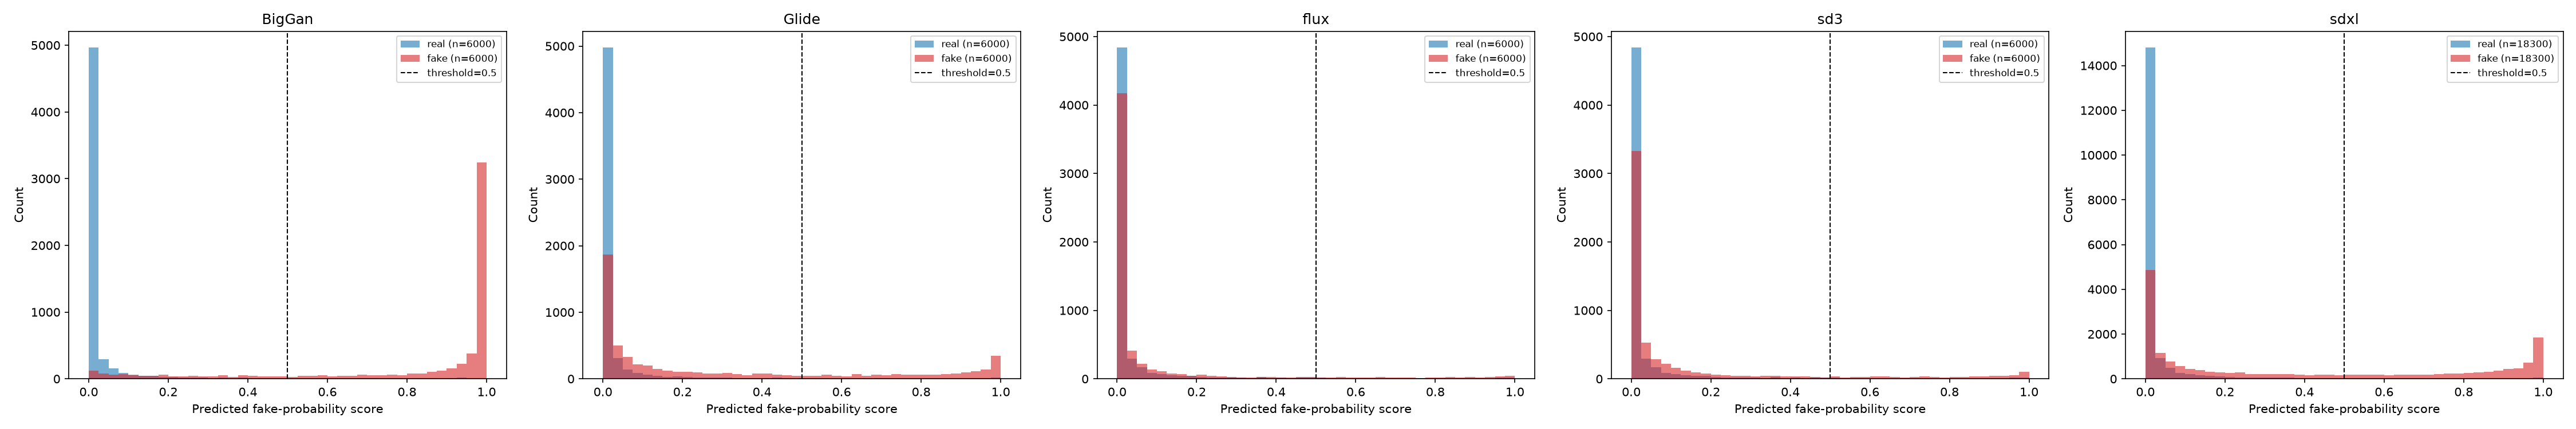
\includegraphics[width=\hsize]{figures/fig_score_dist_ufd.png}
% \caption{UniversalFakeDetect predicted fake-probability scores, real
% (blue) against fake (red), per generator.}
% \label{fig:scoredist}
% \end{figure}

\begin{figure}[t]
\centering
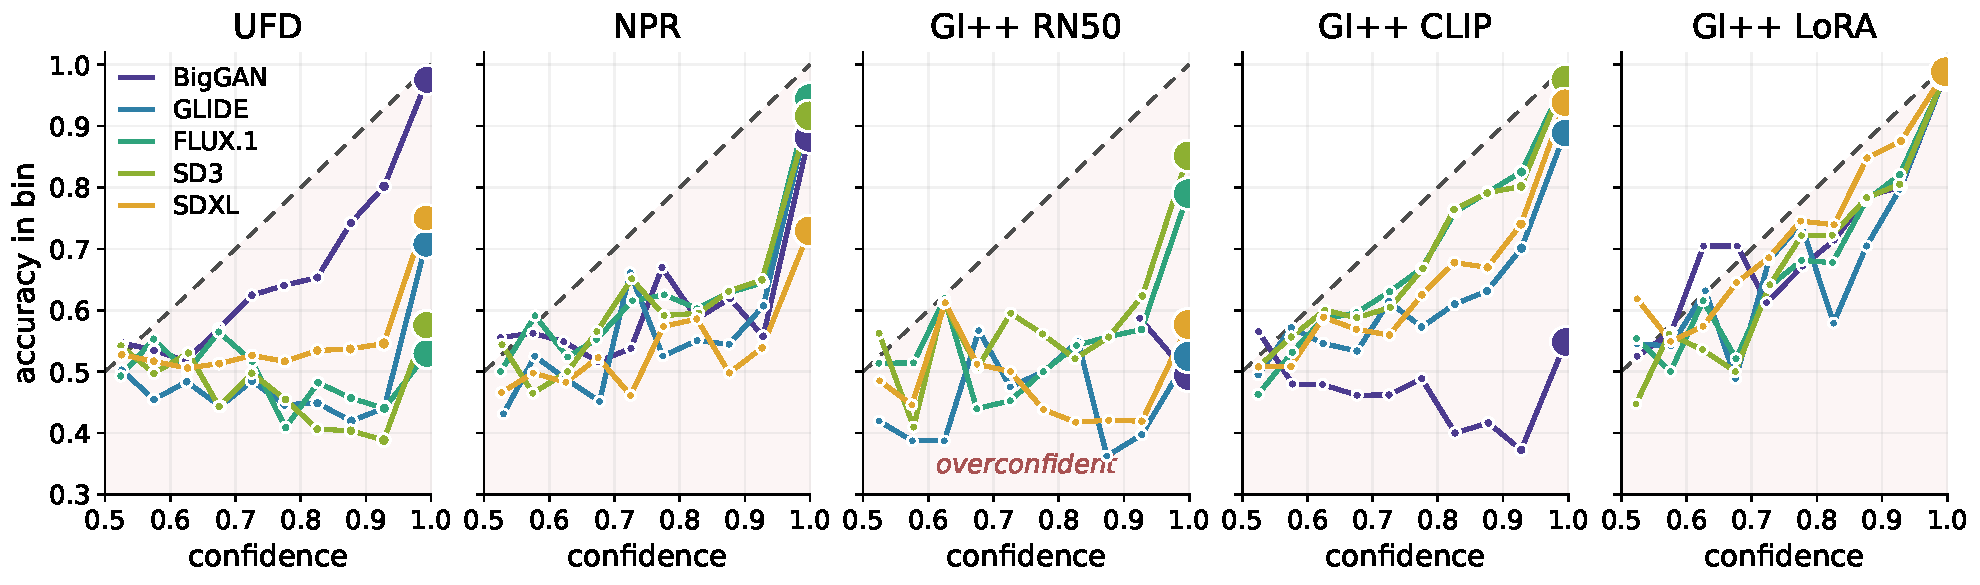
\includegraphics[width=\hsize]{figures/fig_reliability_diagrams.pdf}
\caption{Reliability diagrams, one panel per detector, five generators
each. Confidence is $\max(p,1-p)$ and accuracy is the fraction of images
in the bin classified correctly, the quantities the reported ECE
integrates. Marker area is proportional to the share of images in the bin,
so the dominant mass near confidence 1 is visible rather than averaged
away; bins holding fewer than 25 images are omitted, and the shaded region
below the diagonal is overconfidence. A detector degrading into
uncertainty would move left along the diagonal; these move downward
instead, most visibly the GenImage++ CLIP baseline on BigGAN, whose
largest bin sits at confidence 1.0 and 53\% accuracy.}
\label{fig:reliability}
\end{figure}

Reading that off a histogram is not enough, so we quantify it with
expected calibration error~\cite{guo2017calibration} over 15 equal-width
bins (Table~\ref{tab:auc}) and show the underlying reliability curves in
Figure~\ref{fig:reliability}. The numbers track the failures:
UniversalFakeDetect's ECE is 0.042 on BigGAN, where it works, and 0.439 on
FLUX.1, where it does not, meaning average confidence overstates average
correctness by more than 43 points. A merely uncertain detector would push
scores toward 0.5 and produce a \emph{small} ECE alongside low accuracy;
instead accuracy falls and calibration error rises together. The same
holds for the CLIP baseline on BigGAN (ECE 0.433 at 9.6\% fake-accuracy)
and most starkly for the ResNet-50 on BigGAN, whose ECE of 0.503
accompanies 0.4\% fake-accuracy. CLIP-LoRA is best-calibrated everywhere,
never exceeding 0.020, and is the only panel whose curves track the
diagonal across all five generators.

The diagrams add what the scalar hides: for every failing cell the largest
bin is the rightmost one, so the mass of the distribution sits at maximum
confidence regardless of whether the detector is right, and the curves
separate vertically by generator rather than shifting left. A detector
that fails confidently gives a downstream system no signal that it is
outside its competence, and abstention and human-review routing both
depend on low confidence tracking low reliability.

\section{A preprocessing-driven reproducibility hazard}
\label{sec:discussion}

The disagreement left open in Section~\ref{sec:methods-published} is worth
following, because resolving it turns up a sensitivity that applies to any
cross-paper accuracy comparison in this literature. We first ruled out an
implementation bug: reimplementing the source repository's released
\texttt{kornia}-based preprocessing and running both versions over the
same sixteen images through the same checkpoint gave near-identical
scores, pointing at the preprocessing \emph{choice} rather than a coding
error.

GenImage's BigGAN subset ships fakes at 128$\times$128, unlike every other
generator in the benchmark (GLIDE ships at 256$\times$256), which is the
benchmark's documented convention rather than an artifact of our download.
The released preprocessing resizes every input to 224$\times$224
regardless of native size, so BigGAN's fakes are upsampled nearly twofold
while others are downsampled or left near target. We added a second path
preserving native pixel scale, pasting onto a black canvas rather than
interpolating, and re-ran both checkpoints both ways
(Table~\ref{tab:glidepreproc}). Padding moves the CLIP baseline's overall
accuracy to 61.66\%, within one point of the reported 62.66\%.

Two effects compound: the source paper's accuracy column is almost
certainly overall accuracy across both classes while our first measurement
was fake-only, a metric-definition mismatch on our end, and the resize
direction is a real effect we measured rather than inferred. The same swap
does the opposite to the OMAT checkpoint, dropping it from 99.7\% to
16.3\%, consistent with that paper's note that every fine-tuning strategy
used a fixed resize-to-224 pipeline. We could not close the residual one
point, because GenImage's official distribution is gated behind Baidu
Yunpan and Google Drive with no scriptable, authentication-free access and
the paper's cross-benchmark evaluation script is not among its released
code.

\begin{table}[h]
\caption{Padding versus official upsampling on the two generators whose
native resolution is not 224$\times$224, full evaluation sets. The GLIDE
padding condition is a pure center-crop; the BigGAN one introduces a black
border over 67.3\% of the canvas, so the two are not directly comparable.}
\label{tab:glidepreproc}
\begin{tabular*}{\hsize}{@{\extracolsep{\fill}}llrrr@{}}
\toprule
Generator & Checkpoint / preprocessing & Fake & Real & AUC \\
\colrule
BigGAN (128) & CLIP, upsample & 9.60 & 96.48 & 67.97 \\
BigGAN (128) & CLIP, padding & 25.30 & 98.02 & 90.38 \\
BigGAN (128) & CLIP-LoRA, upsample & 99.70 & 94.82 & 99.70 \\
BigGAN (128) & CLIP-LoRA, padding & 16.28 & 93.12 & 69.13 \\
GLIDE (256) & CLIP, upsample & 69.13 & 96.05 & 94.03 \\
GLIDE (256) & CLIP, padding & 76.93 & 98.20 & 97.44 \\
GLIDE (256) & CLIP-LoRA, upsample & 99.87 & 94.87 & 99.82 \\
GLIDE (256) & CLIP-LoRA, padding & 99.77 & 92.82 & 99.88 \\
\botrule
\end{tabular*}
\end{table}

\subsection{Separating interpolation from border artifacts}
\label{sec:disentangle}

An effect shown on one generator is an anecdote, so we repeated the test
on GLIDE, the only other generator here whose native resolution is not
224$\times$224. For the CLIP baseline it replicates in the same direction
at smaller magnitude (fake-accuracy 69.1\% to 76.9\%, AUC 94.0 to 97.4,
against 9.6\% to 25.3\% and AUC 68.0 to 90.4 on BigGAN), as the resolution
gap predicts. For CLIP-LoRA the two diverge completely: on GLIDE it is
unmoved (99.87\% to 99.77\%), on BigGAN it collapses (99.70\% to 16.28\%).
Our native-resolution path center-crops images larger than 224 and
zero-pads smaller ones, so for GLIDE's 256$\times$256 inputs it is a pure
center-crop with no border, while for BigGAN's 128$\times$128 it produces
a black frame covering 67.3\% of the canvas. The BigGAN collapse is
therefore confounded between the absence of interpolation and a large
out-of-distribution border.

We therefore ran a third condition on BigGAN: a nearest-neighbour upsample
to 224$\times$224, which removes smooth interpolation exactly as padding
does but introduces no border. On matched 2{,}000-image-per-class samples
the two causes separate cleanly. Dropping interpolation alone costs
CLIP-LoRA 37.8 points of fake-accuracy (99.25\% to 61.45\%) while AUC
falls only 1.7, from 99.63 to 97.90: an accuracy collapse with ranking
intact is a threshold problem, the model still ordering generated above
real while the score distribution shifts out from under the fixed cut.
Adding the border is different damage, taking fake-accuracy to 5.30\% and
AUC to 60.36, near enough to chance that no threshold recovers it. This
corrects Section~\ref{sec:finding2}: OMAT's hardening survives a change of
interpolation kernel in ranking terms while losing threshold calibration,
and fails outright only under a distortion with no counterpart in its
training pipeline.

The CLIP baseline moves the opposite way on the same axis: under
nearest-neighbour upsampling its AUC rises to 90.72 from 67.97, so for a
detector never fine-tuned against a fixed pipeline, smooth interpolation
of a 128$\times$128 output is itself destroying signal. Two checkpoints
trained on identical data prefer opposite preprocessing, so no
preprocessing choice is neutral across detectors and a benchmark fixing
one implicitly favours some. A reader comparing published numbers should
treat a resize or crop mismatch as a checkable explanation for an
unexplained gap before concluding either is wrong.

\section{Compression: a robustness failure and a benchmark confound}
\label{sec:compression}

Across all five generators, every generated image in these benchmarks is
distributed as PNG and every real image as JPEG. Real and generated images
therefore differ systematically in compression history, not only in
provenance, and a detector sensitive to compression artifacts can score
well by exploiting that. The bias is documented for GenImage by Grommelt
et al.~\cite{grommelt2024jpeg}, who report that removing JPEG and
image-dimension confounds shifts cross-generator performance by more than
11 points. It also matters on deployment terms, since images reaching a
real detector have usually been re-encoded by whatever platform carried
them.

One experiment answers both questions, run in three conditions on a fixed
FLUX.1 sample of 2{,}000 images per class so that every condition is
paired within a detector (Table~\ref{tab:compression}). \emph{Clean} is
the benchmark as shipped. \emph{Fakes-only} re-encodes the generated
images at JPEG quality 75 and leaves the reals untouched, removing the
format asymmetry and nothing else, so the clean-to-fakes-only drop
estimates how much apparent skill that asymmetry was supplying.
\emph{Both} re-encodes every image, the deployment-style robustness check
and the closest available approximation to a compression-balanced
benchmark.

\begin{table}[h]
\caption{FLUX.1, 2{,}000 images per class, the same sample in every
condition. \emph{Fakes-only} re-encodes generated images at JPEG q75 and
leaves reals as shipped; \emph{both} re-encodes every image. Fake-accuracy
is shared between the two compressed conditions because the generated
images are identical in both, so only AUC separates them. NPR falls below
chance once generated images carry JPEG compression.}
\label{tab:compression}
\begin{tabular*}{\hsize}{@{\extracolsep{\fill}}lcccccc@{}}
\toprule
& \multicolumn{2}{c}{Fake-acc (\%)} & \multicolumn{3}{c}{AUC} \\
Detector & clean & JPEG q75 & clean & fakes-only & both \\
\colrule
UniversalFakeDetect & 7.30 & 6.00 & 61.19 & 60.24 & 55.54 \\
NPR & 98.00 & \textbf{1.50} & 97.10 & \textbf{39.13} & \textbf{50.63} \\
GenImage++ ResNet-50 & 69.45 & 58.00 & 91.27 & 87.02 & 88.48 \\
GenImage++ CLIP & 89.60 & 59.80 & 98.56 & 94.03 & 97.28 \\
GenImage++ CLIP-LoRA & 97.65 & 41.90 & 99.30 & 86.49 & 90.67 \\
\botrule
\end{tabular*}
\end{table}

NPR is the headline in both readings. It is the strongest detector on
clean FLUX.1 by a wide margin (98.0\% fake-accuracy, AUC 97.1), and
compressing only the generated side takes its AUC to 39.13, not merely
chance but below it: the detector then ranks real photographs as more
likely generated than the generated images themselves. That matters for
interpretation. If JPEG re-encoding simply destroyed genuine generative
traces, AUC would fall toward 50 and stop, because destroyed evidence is
absent evidence. An inversion means the quantity NPR reads tracks relative
compression level rather than provenance, which fits its mechanism: it
reads up-sampling artifacts in neighbouring-pixel relationships, and JPEG
quantisation attacks exactly the high-frequency content those live in, so
once the generated side is the more heavily compressed side the sign of
the evidence flips. The clean 98.0\% should not be read as a pure
measurement of generative-artifact detection, though we cannot decompose
it into a provenance part and a compression part, since both explanations
predict a collapse.

The other four detectors set the scale. Removing the format asymmetry
costs the CLIP baseline 4.5 AUC points, the ResNet-50 4.3, CLIP-LoRA 12.8
and UniversalFakeDetect 1.0, against 58.0 for NPR, so the confound
inflates an artifact-based detector by an order of magnitude more than a
semantics-based one. Under full re-encoding their accuracy drops far
exceed their AUC drops (the CLIP baseline loses 29.8 points of
fake-accuracy and 1.3 of AUC), so the ranking still separates the classes
while the fixed threshold no longer sits in the right place, which
recalibration can fix. NPR's cannot, because no threshold helps at an AUC
of 50.6, let alone 39.1: the detector a clean-data leaderboard recommends
is the one that fails most completely on data that has passed through any
normal image pipeline.

Two things limit the damage to the rest of this paper. All five detectors
saw exactly the same images, so the cross-detector comparisons and every
paired test in Section~\ref{sec:significance} hold even if absolute levels
are inflated by a shared bias; and the confound is a property of the
real/fake pairing, so it cannot explain Section~\ref{sec:finding-shape},
where two detectors on identical images produce identical difficulty
orderings at very different levels. Absolute accuracies should nonetheless
be treated as upper bounds, and repeating this study on a
compression-balanced benchmark, such as the debiased GenImage variant
released with~\cite{grommelt2024jpeg}, is the most important single
follow-up.


\section{Recommendations for practitioners}
\label{sec:recommendations}

\begin{enumerate}
\item Choose a detector against the generator families you expect, not
against a headline average: every generator here spans at least 84
accuracy points across five detectors.
\item If you combine detectors, combine across training lineages. Pairing
within a lineage left the shared blind spot in place in every case we
measured, and in one case deepened it from 9.6\% to 0.3\%. Check first
that one strong detector is not better than any pair you can build.
\item Treat confidence as uninformative unless you have calibrated the
detector on data resembling your deployment, since calibration error here
rises with error rate.
\item Pin and publish the preprocessing: resize, crop, interpolation
kernel and normalization statistics, alongside any accuracy you report. A
resize convention alone moved one checkpoint by more than 15 points, and
moved two checkpoints trained on identical data in opposite directions.
\item Evaluate on re-encoded images before deployment. A detector reading
high-frequency artifacts can lose all discriminative power under ordinary
JPEG, and rank-based metrics will show this before accuracy does.
\item Do not use any of these detectors as sole evidence about a specific
image or person.
\end{enumerate}

For benchmark authors, one addition would have saved us days: a small,
scriptable, authentication-free verification subset of a few hundred
images with published checksums, plus the exact preprocessing function and
metric definition behind the headline table.


\section{Limitations}
\label{sec:limitations}

Detector diversity is narrower than ``five detectors'' suggests: three
share a CLIP backbone family, so findings holding across all five are on
firmer ground than those from the CLIP family alone. The set spans 2023 to
2025 and includes two detectors built for the diffusion era, NPR and the
OMAT-hardened CLIP-LoRA, but a genuinely independent family would widen it
further. A diffusion-reconstruction method such as
DIRE~\cite{wang2023dire}, whose signal is neither a CLIP embedding nor a
pixel residual, is the most valuable single addition future work could
make; adding one was outside what an inference-only study on a single
8~GB GPU could complete here. The ensembling test likewise uses one fusion
rule over pairs rather than larger sets, and its worst-generator statistic
is a minimum over five generators and therefore sensitive to which five.

Cross-detector real-accuracy on FLUX.1, SD3 and SDXL is unpaired: because
GenImage++ ships no reals, each run drew its own sample from the shared
162{,}000-image pool and those sets overlap only incidentally (7 of
6{,}000 for FLUX.1 and SD3, 200 of 18{,}300 for SDXL). The fake sets are
identical across all five detectors for every generator, so fake-accuracy
comparisons and every paired test are properly paired, and BigGAN and
GLIDE are matched on both classes. Separately, whether the ImageNet images
behind the GenImage++ checkpoints' training subset overlap our real pools
is unresolved from released materials; it would not affect the
fake-accuracy findings but could slightly inflate real-accuracy for those
checkpoints, and their exact training composition rests on the source
paper's reported methodology, which we could not check against training
logs.

All detectors run at a fixed 0.5 threshold with no tuning, so the accuracy
figures are out-of-the-box behaviour rather than each detector's best
operating point, which is why AUC is reported alongside. On cost, the
three CLIP detectors run at 7.4--7.6 images per second on our 8~GB GPU
while NPR runs at 229--320, roughly 35 times faster. NPR is therefore both
the cheapest detector here and the strongest on the two Diffusion
Transformers under clean data, so the detector chosen on throughput is not
the one chosen from headline accuracy, and neither choice survives
Section~\ref{sec:compression}.


\section{Ethical and dual-use considerations}
\label{sec:ethics}

Documenting where detectors fail is dual-use: the table telling a platform
which detector to avoid also tells an evader which generator to prefer. We
think publication is still right, because the detectors and generators are
already public and these failure modes are discoverable by anyone willing
to run the same inference, the information asymmetry currently runs
against defenders who deploy a single detector assuming a published number
transfers, and our recommendations are defensive rather than evasive. Two
cautions. None of these detectors should be sole evidence in a
consequential decision about a person. And our results are measured on
ImageNet-derived object and scene imagery; we make no claim about images
of people, and face manipulation is out of scope entirely.


\section{Conclusion}
\label{sec:conclusion}

Five pretrained detectors, evaluated on five generators with leakage
verified absent, disagree about which generator is hardest, and the
disagreement is statistically real rather than sampling noise. What
predicts a detector's weak spot is its training distribution, not the
generator's recency: BigGAN, the oldest generator here, is the hardest
case for two detectors and among the easiest for two others.

Two detectors trained on the same data but different architectures rank
the five generators identically while differing 37.6 points in mean
accuracy, which suggests training distribution fixes the shape of a
failure profile and the representation its level. That is a two-detector
observation, so we tested the prediction it makes rather than resting on
it, and it held: a different-lineage partner lifted worst-generator
accuracy from 9.6\% to 62.9\%, while a same-lineage partner of different
architecture pushed the same quantity down to 0.3\%, a separation
significant on every generator. Blind spots travel with training data, and
a different backbone does not move them. What makes those gaps
consequential is that calibration error rises alongside error rate rather
than falling, so a detector leaving its training distribution stays
confident and becomes wrong instead of signalling its own unreliability.

Two measurement findings temper how any of these numbers should be used. A
resize convention rarely specified in released code moves the same
checkpoint by more than 15 points, in opposite directions for two
checkpoints trained on identical data. And because these benchmarks pair
PNG generated images against JPEG reals, re-encoding only the generated
side takes the best clean-data FLUX.1 detector from AUC 97.1 to 39.1,
below chance, while the other four lose between 1 and 13 points; the
detector a clean-data leaderboard recommends is the one least suited to
deployment. Cross-detector comparisons survive both hazards, since every
detector saw the same images, but absolute accuracies should be treated as
upper bounds.


\section*{Acknowledgements}

\appendix
\section{Data and code availability}
\label{sec:availability}

Detector checkpoints and evaluation datasets are the original authors'
public releases, cited in Table~\ref{tab:detectors} and
Section~\ref{sec:methods}. To make the preprocessing and metric
definitions behind every number here checkable rather than described, the
following are released together: the evaluation harness and the exact
command line for each of the 25 detector/generator cells; the per-image
prediction scores (image path, true label, predicted probability) for
every cell, from which the paired tests, calibration computations and the
ensembling analysis are computed; the preprocessing functions for the three
resize conditions of Section~\ref{sec:discussion} and the JPEG conditions
of Section~\ref{sec:compression}, including the normalization statistics
used per detector; and the scripts that regenerate every results table and
the figure from those score files. Everything listed above is available at
\url{https://github.com/MogSquad-FinalYear/BlindSpot}, which also carries the per-image
score files behind every table and the commands that produced them.

\begin{thebibliography}{99}

\bibitem{wang2020cnndetect}
Wang, Sheng-Yu, Oliver Wang, Richard Zhang, Andrew Owens, and Alexei A.\ Efros.
(2020) ``CNN-generated images are surprisingly easy to spot... for now.''
\textit{Proceedings of the IEEE/CVF Conference on Computer Vision and
Pattern Recognition}: 8695--8704.

\bibitem{genimage2023}
Zhu, Mingjian, Hanting Chen, Qiangyu Yan, Xudong Huang, Guanyu Lin, Wei Li,
Zhijun Tu, Hailin Hu, Jie Hu, and Yunhe Wang. (2023) ``GenImage: A
million-scale benchmark for detecting AI-generated image.''
\textit{Advances in Neural Information Processing Systems} \textbf{36}:
77771--77782.

\bibitem{ojha2023universal}
Ojha, Utkarsh, Yuheng Li, and Yong Jae Lee. (2023) ``Towards Universal Fake
Image Detectors that Generalize Across Generative Models.''
\textit{Proceedings of the IEEE/CVF Conference on Computer Vision and
Pattern Recognition}: 24480--24489.

\bibitem{tan2024npr}
Tan, Chuangchuang, Yao Zhao, Shikui Wei, Guanghua Gu, Ping Liu, and Yunchao
Wei. (2024) ``Rethinking the Up-Sampling Operations in CNN-based
Generative Network for Generalizable Deepfake Detection.''
\textit{Proceedings of the IEEE/CVF Conference on Computer Vision and
Pattern Recognition}: 28130--28139.

\bibitem{zhou2025omat}
Zhou, Yue, Xinan He, KaiQing Lin, Bin Fan, Feng Ding, and Bin Li. (2025)
``Breaking Latent Prior Bias in Detectors for Generalizable AIGC Image
Detection.'' \textit{arXiv preprint arXiv:2506.00874}.

\bibitem{flux2024}
Black Forest Labs. (2024) ``FLUX.'' \url{https://github.com/black-forest-labs/flux}.

\bibitem{esser2024sd3}
Esser, Patrick, Sumith Kulal, Andreas Blattmann, Rahim Entezari, Jonas
M\"{u}ller, Harry Saini, Yam Levi, Dominik Lorenz, Axel Sauer, Frederic
Boesel, et al. (2024) ``Scaling rectified flow transformers for
high-resolution image synthesis.'' \textit{Forty-first International
Conference on Machine Learning}.

\bibitem{brock2019biggan}
Brock, Andrew, Jeff Donahue, and Karen Simonyan. (2019) ``Large scale GAN
training for high fidelity natural image synthesis.'' \textit{International
Conference on Learning Representations}.

\bibitem{nichol2021glide}
Nichol, Alex, Prafulla Dhariwal, Aditya Ramesh, Pranav Shyam, Pamela
Mishkin, Bob McGrew, Ilya Sutskever, and Mark Chen. (2021) ``GLIDE:
Towards photorealistic image generation and editing with text-guided
diffusion models.'' \textit{arXiv preprint arXiv:2112.10741}.

\bibitem{podell2023sdxl}
Podell, Dustin, Zion English, Kyle Lacey, Andreas Blattmann, Tim Dockhorn,
Jonas M\"{u}ller, Joe Penna, and Robin Rombach. (2023) ``SDXL: Improving
latent diffusion models for high-resolution image synthesis.''
\textit{arXiv preprint arXiv:2307.01952}.

\bibitem{radford2021clip}
Radford, Alec, Jong Wook Kim, Chris Hallacy, Aditya Ramesh, Gabriel Goh,
Sandhini Agarwal, Girish Sastry, Amanda Askell, Pamela Mishkin, Jack
Clark, et al. (2021) ``Learning transferable visual models from natural
language supervision.'' \textit{International Conference on Machine
Learning}: 8748--8763.

\bibitem{hu2022lora}
Hu, Edward J., Yelong Shen, Phillip Wallis, Zeyuan Allen-Zhu, Yuanzhi Li,
Shean Wang, Lu Wang, and Weizhu Chen. (2022) ``LoRA: Low-rank adaptation
of large language models.'' \textit{International Conference on Learning
Representations}.

\bibitem{peebles2023dit}
Peebles, William, and Saining Xie. (2023) ``Scalable diffusion models with
transformers.'' \textit{Proceedings of the IEEE/CVF International
Conference on Computer Vision}: 4195--4205.

\bibitem{xu2025seed}
Xu, Katherine, Lingzhi Zhang, and Jianbo Shi. (2025) ``Good seed makes good
crop: Discovering secret seeds in text-to-image diffusion models.''
\textit{IEEE/CVF Winter Conference on Applications of Computer Vision}:
3024--3034.

\bibitem{wang2023dire}
Wang, Zhendong, Jianmin Bao, Wengang Zhou, Weilun Wang, Hezhen Hu, Hong
Chen, and Houqiang Li. (2023) ``DIRE for diffusion-generated image
detection.'' \textit{Proceedings of the IEEE/CVF International Conference
on Computer Vision}: 22445--22455.

\bibitem{yan2024chameleon}
Yan, Shilin, Ouxiang Li, Jiayin Cai, Yanbin Hao, Xiaolong Jiang, Yao Hu,
and Weidi Xie. (2024) ``A sanity check for AI-generated image detection.''
\textit{arXiv preprint arXiv:2406.19435}.

\bibitem{qian2020f3net}
Qian, Yuyang, Guojun Yin, Lu Sheng, Zixuan Chen, and Jing Shao. (2020)
``Thinking in frequency: Face forgery detection by mining frequency-aware
clues.'' \textit{European Conference on Computer Vision}: 86--103.

\bibitem{tan2025c2pclip}
Tan, Chuangchuang, Renshuai Tao, Huan Liu, Guanghua Gu, Baoyuan Wu, Yao
Zhao, and Yunchao Wei. (2025) ``C2P-CLIP: Injecting category common prompt
in CLIP to enhance generalization in deepfake detection.''
\textit{Proceedings of the AAAI Conference on Artificial Intelligence}
\textbf{39}: 7184--7192.

\bibitem{rossler2019ff}
R\"{o}ssler, Andreas, Davide Cozzolino, Luisa Verdoliva, Christian Riess,
Justus Thies, and Matthias Nie{\ss}ner. (2019) ``FaceForensics++: Learning
to detect manipulated facial images.'' \textit{Proceedings of the IEEE/CVF
International Conference on Computer Vision}: 1--11.

\bibitem{li2020celebdf}
Li, Yuezun, Xin Yang, Pu Sun, Honggang Qi, and Siwei Lyu. (2020)
``Celeb-DF: A large-scale challenging dataset for deepfake forensics.''
\textit{Proceedings of the IEEE/CVF Conference on Computer Vision and
Pattern Recognition}: 3207--3216.

\bibitem{frank2020frequency}
Frank, Joel, Thorsten Eisenhofer, Lea Sch\"{o}nherr, Asja Fischer, Dorothea
Kolossa, and Thorsten Holz. (2020) ``Leveraging frequency analysis for
deep fake image recognition.'' \textit{International Conference on Machine
Learning}: 3247--3258.

\bibitem{selvaraju2017gradcam}
Selvaraju, Ramprasaath R., Michael Cogswell, Abhishek Das, Ramakrishna
Vedantam, Devi Parikh, and Dhruv Batra. (2017) ``Grad-CAM: Visual
explanations from deep networks via gradient-based localization.''
\textit{Proceedings of the IEEE International Conference on Computer
Vision}: 618--626.

\bibitem{guo2017calibration}
Guo, Chuan, Geoff Pleiss, Yu Sun, and Kilian Q. Weinberger. (2017) ``On
calibration of modern neural networks.'' \textit{International Conference
on Machine Learning}: 1321--1330.

\bibitem{mcnemar1947}
McNemar, Quinn. (1947) ``Note on the sampling error of the difference
between correlated proportions or percentages.'' \textit{Psychometrika}
\textbf{12} (2): 153--157.

\bibitem{grommelt2024jpeg}
Grommelt, Patrick, Louis Weiss, Franz-Josef Pfreundt, and Janis Keuper.
(2024) ``Fake or JPEG? Revealing common biases in generated image
detection datasets.'' \textit{arXiv preprint arXiv:2403.17608}.

\end{thebibliography}

\end{document}
